\section{Task: Post-Process} 
\label{sec:task_postprocess}

This task allows calculation which data sources were active and of minimum/maximum data information, which is required for that later tasks or analysis functions.

\begin{figure}[H]
  \hspace*{-2.5cm}
    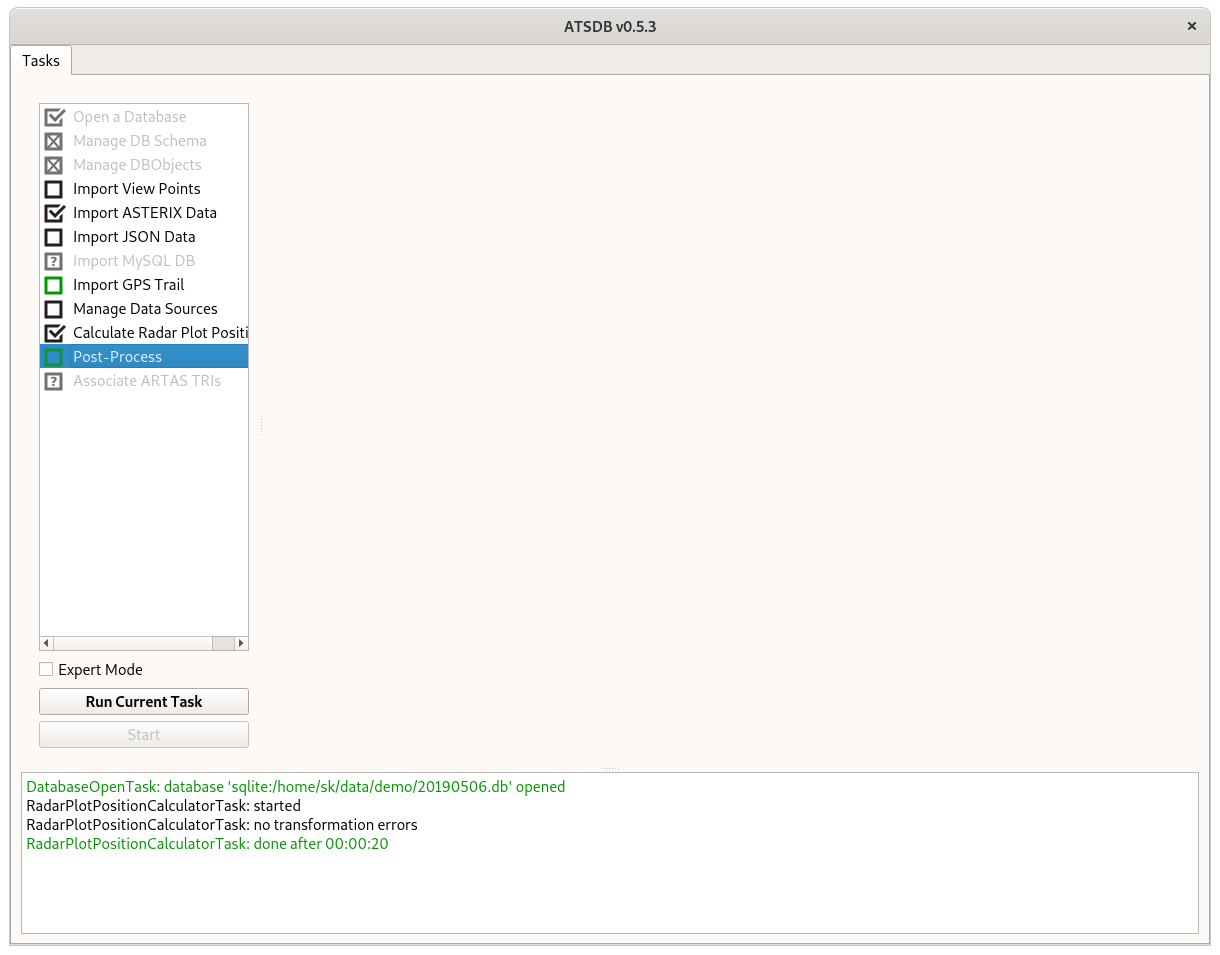
\includegraphics[width=19cm]{figures/db_postprocessing.png}
  \caption{Task: Post-process}
\end{figure}

The following information is generated and stored in the database:

\begin{itemize}  
\item List of all active data sources for all DBOs
\item List with all minima/maxima for all variables of all DBOs
\end{itemize}

This step has to be performed only once for each database, and may take up to a few minutes for large datasets. \\

\subsection{Running}

Using the 'Run Current Task' button the task can be performed. During import a status indication will be shown:

\begin{figure}[H]
  \center
    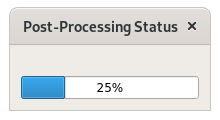
\includegraphics[width=5cm]{figures/postprocess_status.png}
  \caption{Post-processing task status}
\end{figure}

After completion the status window closes and no additional confirmation will be given. \\

\includegraphics[width=0.5cm]{../../data/icons/hint.png} Please \textbf{note} that during this step, no DBObject data itself is changed, but only additional information is generated and stored in separate database tables.
